\title{M\o ller Polarimetry Systematic Error from PITA Feedback }
\author{
        Donald Jones \\
        Temple University\\
 }
\date{\today}

\documentclass[12pt]{article}
\usepackage{hyperref}
\usepackage[english]{babel}
\usepackage{geometry} 
\geometry{letterpaper}
\usepackage[font=footnotesize]{caption}
\usepackage{fullpage}
\usepackage{placeins}
\usepackage{rotating}
\usepackage{graphicx}
\graphicspath{{figures/}}
\usepackage{amssymb}
\usepackage{amsmath}
\usepackage{color}
\usepackage{wrapfig}
\pagecolor{white}
\begin{document}
\maketitle

\abstract{The source laser in the injector at Jefferson Lab is used to produce the polarized electron beam by liberating electrons from a GaAs photocathode preferentially polarized with the same spin as the laser. The laser helicity is flipped rapidly by voltage reversal across a Pockels cell run in quarter-wave mode. Deviations from perfect circular polarization of the laser can produce systematic effects on the beam position, spot size and intensity. These are particularly problematic when they are helicity correlated. The laser is carefully set up to minimize these effects. In particular, the charge asymmetry is zeroed by actively feeding back on the Pockels cell voltages. Since these voltages also control the beam polarization, in principle changing them to mitigate the charge asymmetry could also change the polarization meaning that the polarization during M\o ller measurements might not be reflective of that during the experimental running on average. 

I look at the setup for PREX-2 to see how significant an effect charge feedback might have on polarization. I also look at the potential error for two measurements taken in early August with incorrect Pockels cell set points. I conclude that charge feedback on the PITA voltages introduces an uncertainty in the M\o ller polarization of $<0.1\%$ for both IHWP In and IHWP Out states. There is a difference in sensitivity to PITA voltage changes arising from the fact that laser with IHWP Out was 99.9\% circularly polarized at the photocathode whereas for IHWP In it was only 98.6\%. The average PITA voltages over PREX-2 averaged down close to zero over the experiment for IHWP In. For IHWP Out the average was 5 times larger, but since the circular polarization was higher this resulted in a similar systematic error. Although I infer the effective birefringence of the vacuum window to be $\Delta_{win}=0.115$ radians and to have a significant effect on the laser polarization at the photocathode. I also conclude that the  incorrect Pockels cell voltages during early August are small enough that they do not significantly increase the systematic error already assigned since they happened during a IHWP Out measurement where the sensitivity was smaller. Finally, I conclude that in order to limit systematic uncertainty in M\o ller polarization from charge feedback induced polarization changes, the laser should be set up to have $>$99.9\% circular polarization at the photocathode. }
\section{Introduction}
The source laser in the injector at Jefferson Lab is used to produce the polarized electron beam by liberating electrons from a GaAs photocathode preferentially polarized with the same spin as the laser. Deviations from perfect circular polarization of the laser can produce systematic effects on the beam position, spot size and intensity. The laser polarization is rapidly flipped (at 30 Hz - 1 kHz) to reverse the electron beam polarization and if these deviations are correlated with the laser polarization they become sources systematic error for experiments such as parity experiments whose physics measurements are scattering asymmetries \cite{Paschke2007}.  Figure \ref{fig:laser_schematic} shows a schematic of the laser apparatus for producing polarized beam.

\begin{figure}[hb]
\begin{center}
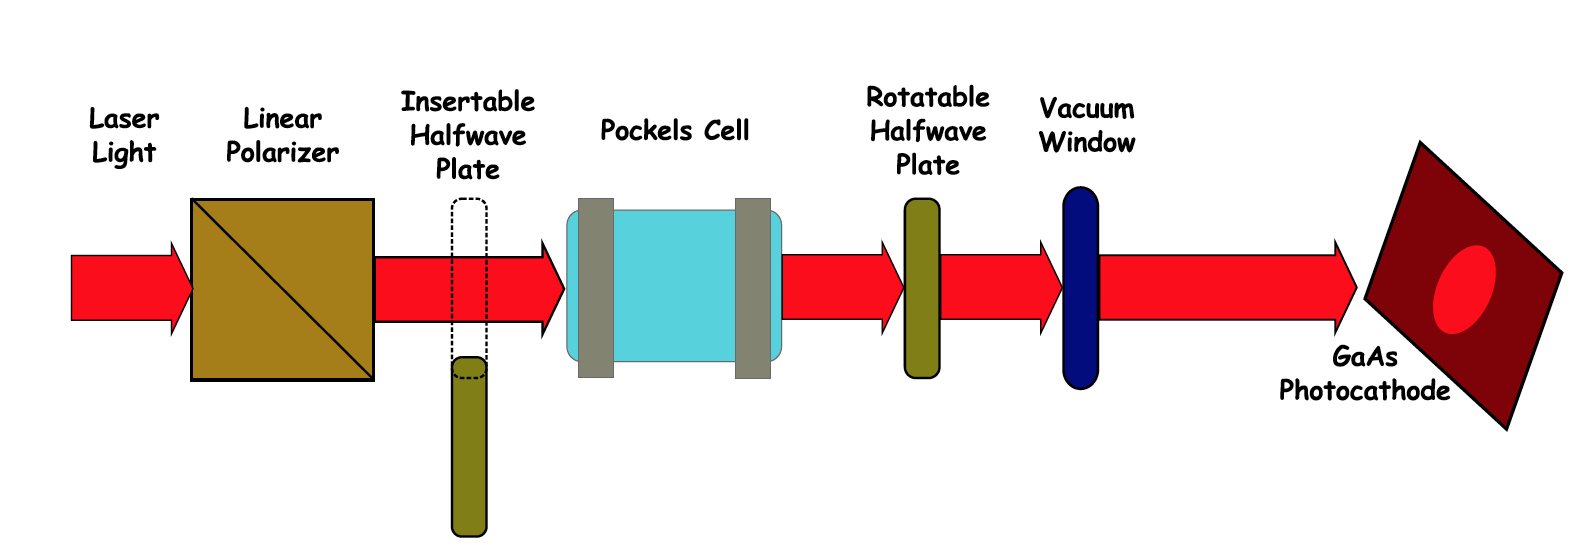
\includegraphics[width=0.8\textwidth]{laser_schematic.png}
\caption{\label{fig:laser_schematic} Schematic illustrating the key elements of the laser setup for producing the polarized electron beam at Jefferson Lab.}
\end{center}
\end{figure}
The fast reversal of the polarization is accomplished with a Pockels cell in quarter wave mode, where the relative $E_x$, $E_y$ phase difference is $\pm\pi/2$ (or alternately $\lambda/4$) and is accomplished by reversing the sign of the voltage on the cell. The GaAs photocathode is known to have an analyzing power for linearly polarized light producing more charge for one state than the other (eg. horizontal and vertical) with an {\it a priori} undetermined analyzing axis. Since this residual linear polarization can lead to a helicity correlated charge asymmetry, great deal of effort is put into producing 100\% circularly polarized light at the photocathode. From the diagram in Fig. \ref{fig:laser_schematic} you can see there are a number of optical elements between the linear polarizer and the photocathode all with the potential to contribute to the total birefringence. Ideally, one would like the total birefringence to be $\pm\lambda/4$ to produce perfectly circular light. However, the half-wave plate(s) may not produce a perfect $\lambda/2$ delay and the vacuum window can contribute an unknown birefringence. Morever, the Pockels cell may have a non-zero latent birefringence with no voltage applied from crystal stresses. These polarization effects can cause a total residual birefringence that is more or less than the desired $\lambda/4$. This fixed sign phase advance (or lag) is called the $\Delta$ phase and adds to both helicity states $\pm\pi/2-\Delta$ leading to a residual linear polarization of equal size but opposite axis for opposite helicities (Pockels cell voltages). This can be illustrated using the Jones matrix formalism by putting a nearly circularly polarized beam through a linear polarizer with its axis at an arbitrary angle $\theta$ measured counterclockwise from the horizontal x-axis. Eq. \ref{eq:jones} subtracts a $\Delta$ of birefringent phase from both states.
\begin{equation}
\label{eq:jones}
R_\Delta(L_\Delta)=
\begin{bmatrix}
\cos^2\theta & \cos\theta\sin\theta\\
\cos\theta\sin\theta & \sin^2\theta
\end{bmatrix}
\frac{1}{\sqrt{2}}
\begin{bmatrix}
1\\
-(+)[i\cos\Delta+\sin\Delta]
\end{bmatrix},
\end{equation}
where $R_\Delta(L_\Delta)$ are the nearly right(left) circularly polarized states.The light transmitted through the linear polarizer after simplification is given by
\begin{equation}
\left| R_\Delta(L_\Delta)\right|^2= \frac{1}{2}\left[1-(+)\sin\Delta\sin2\theta\right].
\end{equation}
The offset in the this equation is from circularly polarized light and the sinusoidal modulation is from linearly polarized light. The linear and circular polarizations under the assumption of 100\% polarized light can be obtained from the transmitted intensity of the rotating linear polarizer as follows: 
\begin{equation}
\label{eq:dolp}
LP = \frac{\textrm{Amplitude}}{\textrm{Offset}}=\left|\sin\Delta\right|, ~~~~~CP = \sqrt{1-LP^2}.
\end{equation}
From this equation you can see that the right and left states have orthogonal residual linear polarization vectors with the right state having a maximum at $\theta=3\pi/4$ and the left at $\theta=\pi/4$. \textbf{Notice there is an ambiguity of the sign of the $\Delta$ w.r.t. to a given LP.} Notice also, the characteristic $2\theta$ frequency in the LP scan arising due to the $\Delta$. Combining the two equations in Eq. \ref{eq:dolp} one obtains 
\begin{equation}
\label{eq:docp}
CP = \sqrt{1-\sin^2\Delta}\approx1-\frac{\Delta^2}{2}, ~~~\Delta<<1.
\end{equation}
The delta term will in general show up as a charge asymmetry unless mitigated by careful laser preparation. One of the knobs for removing charge asymmetries on the beam is to change the positive and negative voltages on the Pockels cell to effectively cancel the $\Delta$ phase advance. This technique has been employed in active feedback mode during all recent parity violation experiments at Jefferson Lab. The feedback utilizes predetermined ``PITA" slopes $(dV/dA_q)$ to average the charge asymmetry to zero by actively adjusting Pockels cell voltages\footnote{PITA which stands for "Phase Induced Transmission Asymmetry" refers to the difference in photocathode current due to relative differences in the phase advance  of the opposite helicity states.}. However, since polarization effects are not the only cause of charge asymmetry, in principle, one could use this PITA feedback to mitigate something not directly related to the delta phase. Furthermore, since adjusting PITA voltages effectively is tweaking the laser polarization, it is prudent to ask how large these tweaks can be before the laser polarization is being significantly altered. The answer to this, of course, depends not only on the relative size of the tweaks but also on how close to being centered on 100\% CP you are when you start making tweaks around the central value. 
\section{Data from PREX-2}
As previously mentioned, the $\Delta$ term can arise from contributions of the IHWP, RHWP, the Pockels cell and the vacuum window. These contributions are additive and can be either sign meaning they can potentially cancel each other out. \footnote{This is an oversimplification in that birefringent elements are characterized by both a retardance and an azimuthal fast axis angle and are thus not directly additive. For example, two birefringent elements with 0.1 radians of retardance but opposite sign will not cancel each other out unless their axes are aligned. Including the angle, however, is not required for the study of the effect of birefringent elements on the polarization of the electron beam. For further details see the Appendix.} After the completion of PREX-2, measurements of the laser polarization on the laser table upstream of the vacuum window were made. These measurements can be found in the DOP spreadsheet in the log entry  https://logbooks.jlab.org/entry/3730981. These directly measure the degree of linear polarization (DOLP) which, as I showed in Eq. \ref{eq:docp} is approximately equal to $\Delta$. It is not straightforward to directly measure the vacuum window birefringence given the difficulty of putting measuring devices between it and the photocathode. Thus, direct measurements of laser polarization that occur on the laser table of necessity omit this additional source of birefringence; however, its size can be inferred from measurements of the laser polarization for both IHWP states. I only utilized rows containing the labels ``Flip script", ``Flip script in/in" or ``Flip script out/out" since these are supposed to be near central value where the PITA voltages were set and around which PITA corrections were made. From the average of these I obtain
\begin{equation}
\Delta_{IN}\approx\langle DOLP_{IN} \rangle=\pm0.053 ~~~ \textrm{and}~~~ \Delta_{OUT}=\langle DOLP_{OUT} \rangle=\pm0.164
\label{eq:docp_in}
\end{equation}
and 
\begin{equation}
\label{eq:docp_out}
\langle DOCP_{IN} \rangle=\pm0.9985 ~~~ \textrm{and}~~~ \langle DOCP_{OUT} \rangle=\pm0.9865
\end{equation}
To infer the birefringence of the vacuum window I note that the difference between the electron beam polarization measured for IHWP Out and In is $1-P_{IN}/P_{OUT}\approx 0.013.$ Using the fact that the phases are additive and assuming this 1.3\% difference comes from the vacuum window contribution $\Delta_{vw}$ gives the following approximate equation:
\begin{equation}
\label{eq:soln}
\begin{split}
0.013&=\sqrt{1-(\Delta_{OUT}+\Delta_{vw})^2}-\sqrt{1-(\Delta_{IN}+\Delta_{vw})^2}\\
~&\approx\frac{\left(\Delta_{IN}+\Delta_{vw}\right)^2}{2}-\frac{\left(\Delta_{OUT}+\Delta_{vw}\right)^2}{2}
\end{split}
\end{equation}
where the signs of the $\Delta s$ can be either positive or negative. Upstream of the vacuum window the polarization of IHWP Out is 1.2\% smaller than that of IN whereas downstream of the vacuum window it is nearly reversed with Out being 1.2\% greater than IN.  This suggests that $\Delta_{OUT}$ and $\Delta_{vw}$ are opposite sign and for the IHWP Out state nearly cancel.  Let's choose to assign $\Delta_{OUT}>0$ and $\Delta_{vw}<0$. Substituting in to Eq. \ref{eq:soln} yields
\begin{equation}
\label{eq:solve}
dP=P_{OUT}-P_{IN}=0.012 \approx \frac{\left(\pm0.053+\Delta_{vw}\right)^2}{2}-\frac{\left(0.164+\Delta_{vw}\right)^2}{2},
\end{equation}
with solutions of either $\Delta_{vw}=-0.110$ or $\Delta_{vw}=-0.216$. Caryn Palatchi has said that she has inferred a window birefringence in the range of 0.10 to 0.15 so I will take the smaller of the two giving a window birefringence of 0.110 radians or 6.6 degrees and $\Delta_{IN}=-0.053$.  \textbf{Substituting these into Eqs. \ref{eq:docp_in} and \ref{eq:docp_out}  gives the circular polarization at the photocathode during PREX-2 of }
\[DOCP_{OUT}=\sqrt{1-(0.164-0.110)^2}=0.9985
\]
 and 
 \[DOCP_{IN}=\sqrt{1-(-0.053-0.110)^2}=0.9866.
 \]

A certain degree of uncertainty exists for each of the parameters ($\Delta_{IN}, \Delta_{OUT}$, and $dP$) in Eq. \ref{eq:solve}. The In/Out polarization difference is known to 0.14\% and we will assume the linear polarization is known to $\pm$2\%. This gives an uncertainty of 0.023 on $\Delta_{vw}$.

Armed with this information we are now ready to evaluate the systematic error for Moller polarimetry arising from the PITA voltages.

The Pockels cell voltages associated with $\pm\lambda/4$ operation are $V\sim\pm12760$. It is typical to have $\pm300$~V adjustments to this from the PITA feedback. This implies that the $\Delta$ term can fluctuate by $\pm\frac{\pi}{4}\left(\frac{300}{12670}\right)=\pm0.04$. However, the actual PITA voltages are saved as a function of time via the EPICS archiver at Jefferson Lab.  Figure \ref{fig:pitavst} shows the PITA voltages as a fraction of the quarter wave voltage taken from the EPICS archiver between August 1 and the end of the experiment on September 8. The data is taken only from times when the current was above 40~$\mu$A. July was neglected since we don't have reliable polarimetry before August. Averaging these data yields on average the deviation from the setpoint was -22 units for IHWP In and -125 units in the units where the $\lambda/4$ setpoint is 12670. \footnote{In units of quarter wave voltage this is -0.172\% for IHWP In and -0.986\% for IHWP Out.}$\frac{22}{12670}\times\frac{\pi}{2}=0.003$ radians of change in $\Delta$ for IHWP In and likewise $\frac{125}{12670}\times\frac{\pi}{2}=0.016$ radians for IHWP Out. Direct addition or subtraction of this from the $\Delta$ changes the polarization by 
\[
\frac{\delta P_{PITA}(IN)}{P}=\pm0.05\% 
\]
\[
\frac{\delta P_{PITA}(OUT)}{P}=\pm0.09\%.
\]
\begin{figure}
\centering
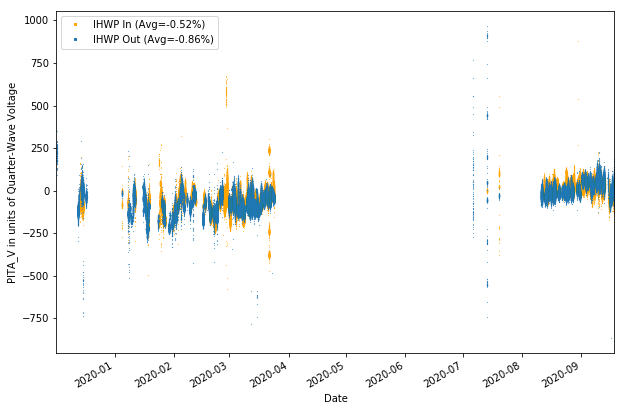
\includegraphics[width=1\textwidth]{pitavst.png}
\caption{\label{fig:pitavst}PITA voltages for IHWP In and Out states given as a fraction of the quarter wave voltages over time. The average is -0.172\% for In and -0.986\% for Out.}
\end{figure}
This assumes that all M\o ller polarization measurements were taken at the PITA setpoints for IHWP In and Out. In fact, this may not be the case since the flipper script is only run (which sets PITA to the setpoints) when the IHWP state is changed. However, it seems reasonable that comparison of the average deviation from the setpoint would serve as an upper bound on the deviations from the PITA values during M\o ller measurements.

During two M\o ller measurements in early August (4th and 10th) the IHWP Out polarization measurements were taken without running the flipper script to reset the PITA voltages to the new setting. Therefore, the IHWP Out measurements were taken at the IHWP In settings, a total of $-970-303=-1273$~V off or about 10\% of the $\pi/2$ voltage introducing an additional $\Delta$ of 0.16 according to the calculation, which I will refer to as $\Delta^{\prime}$. We can calculate how much we expect this to change the laser polarization; however, we also have direct measurements of this change which are always preferred. Data taken on the laser table with IHWP Out at the In PITA voltages shows that the circular polarization goes from 98.9\% at the correct setting to 99.9\% at the incorrect setting where the polarization measurement was taken (compare lines 5 and 9 of the DoP spreadsheet available at https://logbooks.jlab.org/entry/3730981). The LP  goes from 14.8\% at the correct setting to 3.9\% at the incorrect setting implying a measured $\left|\Delta^{\prime}\right|=(0.148\pm0.039)$ which is either 0.19 or 0.11 depending on the sign.  Perhaps a more accurate estimate is obtained from the data in Fig. \ref{fig:dolpvspita_out} where DOLP versus PITA voltage is plotted. Although the data are noisy an overall trend can be seen. The slope of the line gives 0.96e-4~radians/V yielding $\left|\Delta^\prime\right|=0.12$ for 1273~V. This is significantly less than the expected 1.24e-4~radians/V for a total $\left|\Delta^\prime\right|=0.16$ expected from calculation.   I conclude that the sign of $\Delta^{\prime}$ has the opposite sign to $\Delta_{OUT}$ and the same sign as $\Delta_{win}$ because both $\Delta^{\prime}$ and $\Delta_{win}$ result in higher polarization when included. So this means $\Delta^{\prime}$ is likely somewhere between -0.12  and -0.16 in my convention. Adding the three phases gives $DOCP_{OUT@IN PITA}=\sqrt{1-(0.164-0.115-\Delta^{\prime})^2}=0.9975~\textrm{to}~0.9938$. This implies that the polarization was as much as 0.1\% to 0.5\% lower during the measurement than at the proper setting. If the offset PITA voltage offset had been the opposite sign ($\Delta^{\prime}$ between +0.12 and +0.16) we would have been at 0.986 to 0.978 which is 1-2\% low, and we certainly would have noticed that large a difference. \textrm{Using these calculations I conclude that we do not need to make any correction for the incorrect PITA settings for IHWP Out on Aug 4 and 10. The impact of this small systematic error in these measurements is negligible compared to the 0.2\% systematic already assigned to IHWP Out measurements.}\footnote{The measurements affect 2 points out of 12 so even assigning the larger systematic error of 0.5\% to these would only bring the total IHWP Out systematic error from PITA to 0.22\%.} It would have been a different story if the settings were incorrect for IHWP In instead. 
\begin{figure}
\centering
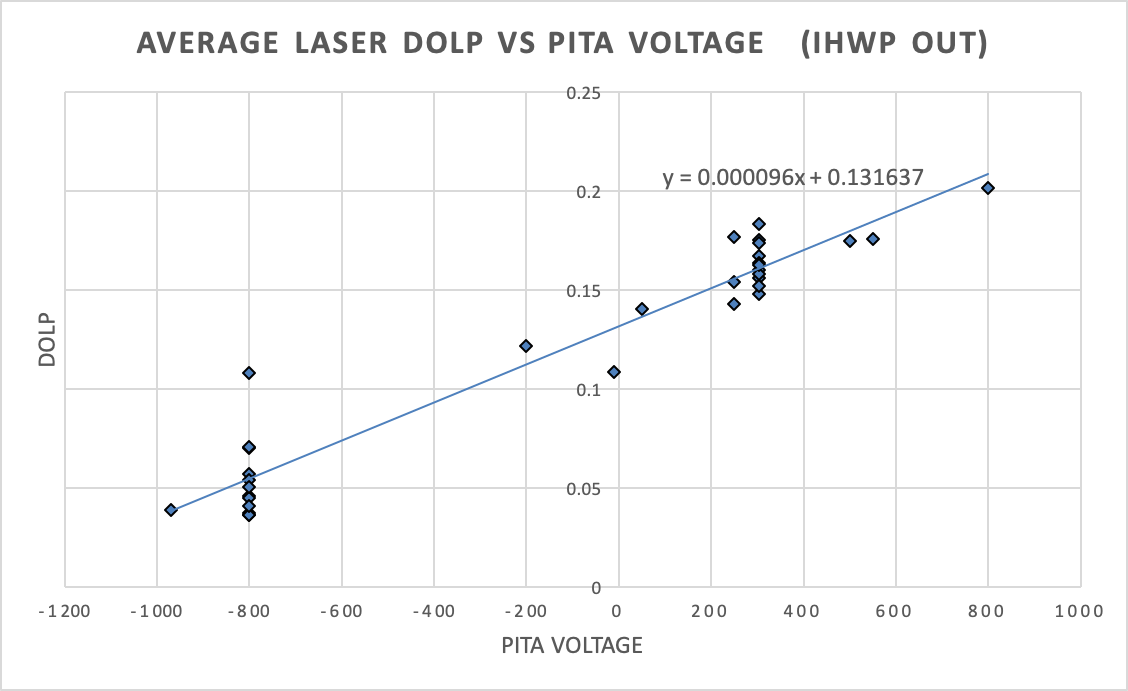
\includegraphics[width=0.8\textwidth]{DOLPvsPITA_out.png}
\caption{\label{fig:dolpvspita_out} DOLP versus PITA voltage for IHWP Out taken on the laser table after PREX-2. The slope is 0.94e-4 radians/V.}
\end{figure}
\begin{figure}
\centering
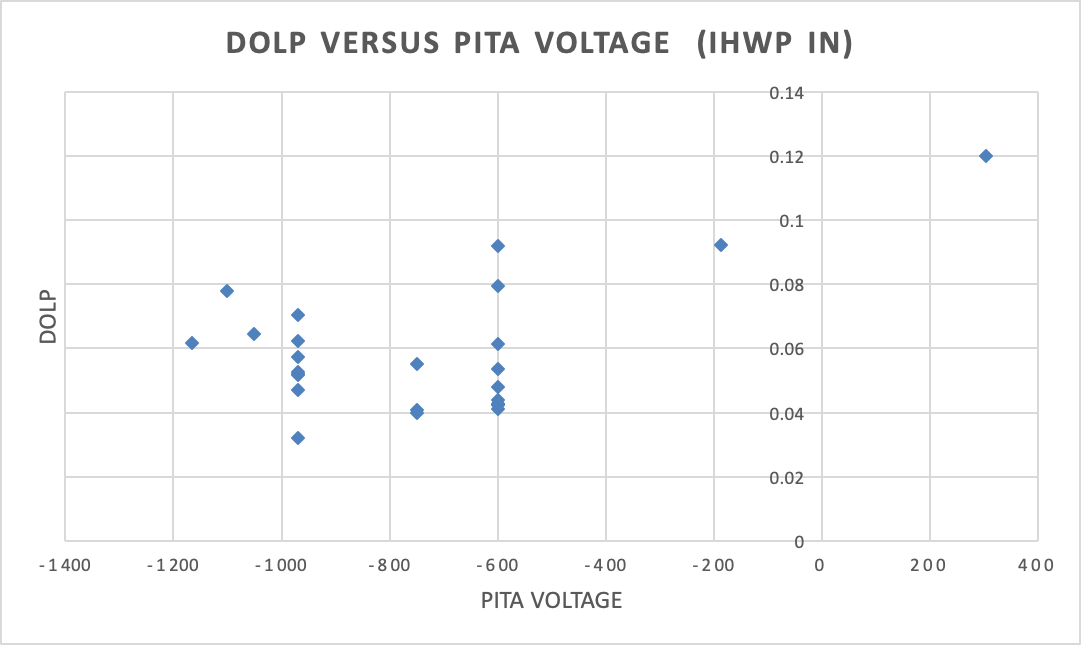
\includegraphics[width=0.8\textwidth]{DOLPvsPITA_in.png}
\caption{\label{fig:dolpvspita_in} DOLP versus PITA voltage for IHWP In taken on the laser table after PREX-2. No fit is performed because the data are dominated by noise down near 0 DOLP.}
\end{figure}

Finally, it is worth noting that even if the laser is set up to be 99.9\% circularly polarized (i.e. $LP=4.5\% $), fluctuations in PITA voltages of $\pm$300~V can induce polarization changes greater than 0.2\%. This could be a significant systematic error in M\o ller polarimetry during MOLLER that Compton would not be sensitive to.

\section{Conclusions}
The following list summarizes the findings of this study.
\begin{enumerate}
\item{For small birefringent phase shifts $\Delta$ away from perfect circular polarization at phase difference of $\pi/2$, the residual linear polarization is equal to the extra phase shift $\left|\Delta\right|$. This sign ambiguity can have significant impact on conclusions and should  be determined. }
\item{Using the laser polarizations measured on the table upstream of the vacuum window combined with the beam polarization measurements during PREX-2, I infer an effective vacuum window birefringence of $\Delta_{vw}=0.115$ with an undetermined uncertainty. For details on what is meant by an effective vacuum window birefringence see Appendix \ref{app:a}.}
\item{Laser polarization measurements on the table showed the laser polarization lower for IHWP Out @98.7\% than for In @ 99.9\%. Using the $\Delta_{vw}$ from (2) we see this was nearly reversed after the laser went through the vacuum window to give 99.9\% for IHWP Out and 98.6\% for In.}
\item{The further you are from 100\% circular polarization the more sensitive you are to changes in the total $\Delta$ from PITA voltage feedback. M\o ller measurements were taken for the most part at the correct PITA voltage set points for both IHWP states (as set by the flipper script). However, feedback on $A_q$ often walked the PITA voltages hundreds of steps from these set points during running meaning the measured polarization was not necessarily equal to that of the experimental running conditions. However, during PREX running the PITA voltages  averaged very close to the PITA set points creating small systematic errors of less than 0.1\% for both IHWP states. This fortuitous averaging down is not guaranteed. For simplicity, a systematic error of 0.1\% will be assigned for both IHWP states.}
\item{Although there were two measurements taken in early August where the flipper script was not run for IHWP Out measurements, the additional systematic uncertainty is negligible. This would not be the case if the voltage offsets were opposite sign or if it happened during an IHWP In measurement.}
\item{Laser measurements on the table upstream of the vacuum window showed equal laser polarization between right and left helicity states to high precision although there was non-negligible DOLP.  Addition of the extra $\Delta_{vw}$ term does not change this equality although it will in general change the DOLP.}
\item{It is critical to set up the laser to be 100.0\% circularly polarized for both IHWP states in order to keep PITA corrections from changing the polarization of the beam at $0.1$\% level.}
\end{enumerate}
\FloatBarrier
\appendix
\section{\label{app:a}Dealing with an angle between axes of birefringent elements}
As noted in the text, when dealing with multiple birefringent elements, the total linear polarization is a function not only of their retardance, $\Delta$, but also of the relative angle of their fast axes. To demonstrate the effect this will have on the analysis of this technote where we simply added or subtracted the $\Delta$s without reference to any angle we will utilize the Jones calculus formalism. With anything but the simplest system, the algebra becomes quickly unwieldy and difficult to maneuver into an analytic expression. Thus, we will rely on numerical analysis . The Jones matrix of a linear retarder with retardance $\Delta$  and fast axis at an angle $\theta$ relative to the positive x-axis is given by \cite{1987Gil}:
\begin{equation}
\label{eq:bif_arb}
e^{\frac{-i\Delta}{2}}
\begin{bmatrix}
\cos^2\theta +e^{i\Delta}\sin^2\theta         & \left(1-e^{i\Delta}\right)\cos\theta\sin\theta \\
 \left(1-e^{i\Delta}\right)\cos\theta\sin\theta  & \sin^2\theta +e^{i\Delta}\cos^2\theta
\end{bmatrix}
\end{equation}
In this equation positive $\Delta$ decreases the phase of y relative to x and vice versa. In the laser setup, the Pockels cell fast axis is set at 45$^\circ$ to the horizontal. For the sake of simplicity in this analysis I arbitrarily assume that there is a $\Delta$ component on the beam upstream of the vacuum window that comes from the Pockels cell being not quite a perfect quarter-wave plate. In this case I start with left circularly polarized light and give a small extra retardance $-\Delta$ as follows:
\begin{equation}\frac{e^{i\Delta}}{\sqrt{2}}
\begin{bmatrix}
1\\
i\\
\end{bmatrix}=\frac{1}{\sqrt{2}}
\begin{bmatrix}
1\\
-\sin\Delta+i\cos\Delta\\
\end{bmatrix}.
\end{equation}
I then take this state and multiply it by the matrix in Eq. \ref{eq:bif_arb} to get the total state including the vacuum window birefringence at an arbitrary angle relative to the axis of the $\Delta$. This resulting state I then analyze using a linear polarizer which in the Jones formalism is:
\begin{equation*}
\begin{bmatrix}
\cos^2\phi     & \cos\phi\sin\phi\\
\cos\phi\sin\phi & \sin^2\phi
\end{bmatrix},
\end{equation*}
giving the transmitted vector as a function of the azimuthal rotation angle of the polarizer. The norm-square of the transmitted vector gives the intensity as a function of angle from which the degree of linear polarization (DOLP) can then be determined by a sinusoidal fit to intensity versus angle. The DOLP is the amplitude divided by the offset term or as often stated it is the difference between maximum and minimum transmitted intensities divided by their sum. 
Figure \ref{fig:pita_vs_angle} shows the results of repeating this analysis to find DOLP for several values of vacuum window birefringence ($\Delta_{vw}$) over a range of relative angles between the birefrigence axis of the vacuum window and the upstream optics.
\begin{figure}
	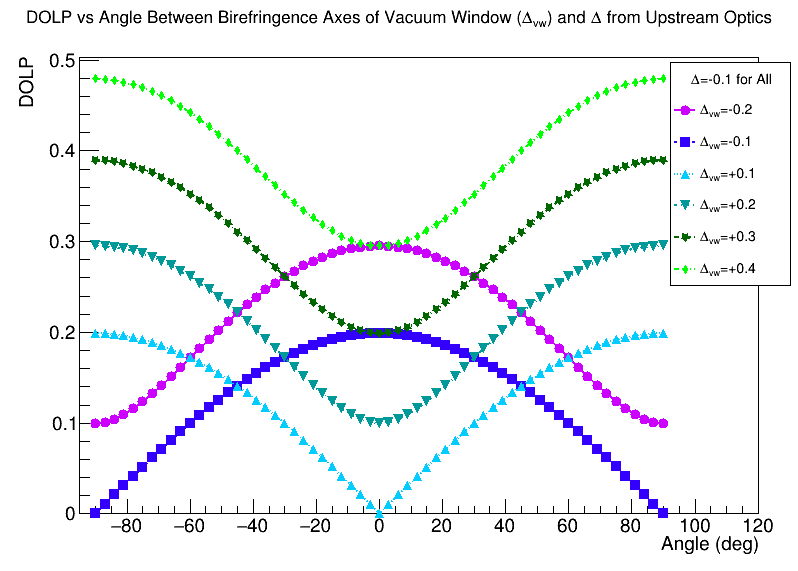
\includegraphics[width=0.9\textwidth]{Vacuum_window_delta_vs_angle.png}
	\caption{\label{fig:pita_vs_angle}Linear polarization induced by the vacuum window birefringence $\Delta_{vw}$ shown as a function of the angle between its axis of birefringence and the axis of the $\Delta$ from upstream optics. For all cases the $\Delta$ component from upstream of the vacuum window is $-$0.1 radians.}
\end{figure}

The following conclusions can be taken away:
\begin{itemize}
\item{The function of DOLP versus relative angle is not a simple sinusoid but is a complicated periodic function of both relative angle and the magnitude of the birefringence.}
\item{The only way to get perfect circular polarization is to have an optical element with the same magnitude of birefringence at either 0$^\circ$ or 90$^\circ$. }
\item{When the axes  of birefringence are aligned or 90$^\circ$ to each other, the $\Delta$s simply add or subtract. These two alignments create the states of maximum and minimum linear polarization. Although we don't have access to a simple algebraic expression, the maximum and minumum values of DOLP are simple expressions and at least provide us with a best and worst case scenario for a given vacuum window birefringence.}
\item{As expected when $\Delta_{tot}$ is no longer small, the approximation $DOLP\approx\Delta_{tot}$ is no longer valid and the exact relation must be used $DOLP=\sin\Delta_{tot}$.}
\end{itemize}

Now let's apply these conclusions to the problem of unknown vacuum window birefringence $\Delta_{vw}$. Eq. \ref{eq:soln} assumes the $\Delta$s are directly additive which is the same thing as assuming they either have their axes aligned or normal to each other. This is not an issue for the electron beam polarization analysis since it relies on measurements of linear polarization of the laser and measurements of beam polarization. It is an issue if you actually need to know the magnitude of the vacuum window retardance but don't know the angle. In a sense $\Delta_{vw}$ is an effective vacuum window retardance since it is interpreted as the retardance that would create the given conditions (In/Out difference together with measured laser polarizations) if the birefringent axes were aligned. One could express the true birefringence as a function of our effective $\Delta_{vw}$ as 
\[
\Delta_{vw}=\Delta^{\textrm{true}}_{vw}f(\delta),
\]
where $\delta$ is the relative angle between the birefringent axes and $f(\delta)$ is an even periodic function with a range between $-1$ and $+$1 and a period of $\pi$. Thus, when the axes are aligned and normal we get the two values of $\Delta_{tot}=\Delta\pm\Delta^{\textrm{true}}_{vw}$.  If one knew the relative angle of the birefringent axis of the vacuum window, one could construct $f(\delta)$ using the Jones formalism as done in Fig. \ref{fig:pita_vs_angle} and then find the true value of the retardance $\Delta^{\textrm{true}}_{vw}$. If the angle is not known, given value of measured $DOLP\approx\Delta_{vw}$ has a range of possible birefringences from $\Delta_{vw}-\Delta$ to $\Delta_{vw}+\Delta$. You can see this explicitly in Fig. \ref{fig:pita_vs_angle} where, for example, a measured DOLP of 0.1 could correspond to $\Delta^{\textrm{true}}_{vw}=-0.2@\pm90^{\circ}$, $\Delta^{\textrm{true}}_{vw}=+0.2@0^{\circ}$, $\Delta^{\textrm{true}}_{vw}=+0.1@\pm32^{\circ}$ or $\Delta^{\textrm{true}}_{vw}=-0.1@\pm60^{\circ}$. Therefore, the upstream $\Delta_{IN}=0.053$ for the IHWP In laser state upstream of the vacuum window in addition to the calculated $\Delta_{vw}=0.115$, can be used to place limits on the range of the vacuum window birefringence: $\Delta^{\textrm{true}}_{vw}=0.115\pm0.053$. 
\newpage

%\bibliographystyle{abbrv}
\bibliographystyle{unsrt}
\bibliography{bibliography}
\end{document}
